\documentclass{nature3}
\usepackage{graphicx}
\usepackage{float}
\usepackage{verbatim}
\usepackage{hyperref}
\usepackage{amsmath}
\usepackage{amssymb}
\usepackage{aas_macros_nature}
\usepackage{lineno}

\linespread{1.0}
\linenumbers % turn line numbering on or off

\newcommand{\starname}{TIC 141146667}

\newcommand{\farcm}{\mbox{\ensuremath{.\mkern-4mu^\prime}}}%    % fractional arcminute symbol: 0.'0
\newcommand{\farcs}{\mbox{\ensuremath{.\!\!^{\prime\prime}}}}%  % fractional arcsecond symbol: 0.''0

\newcommand{\kms}{\ensuremath{\rm km\,s^{-1}}}
\newcommand{\ms}{\ensuremath{\rm m\,s^{-1}}}

\renewcommand*{\thefootnote}{\fnsymbol{footnote}}

%%%%%%%%%%%%%%%%
% INSTITUTIONS %
%%%%%%%%%%%%%%%%
\newcommand{\carnegie}{Observatories of the Carnegie Institution for Science, Pasadena, CA 91101, USA}
%%%%%%%%%%%%%%%%

%%%%%%%%%%
% VALUES %
%%%%%%%%%%
% NOTE: might need to be ingested before submission 
\newcommand{\stteff}{YYYY}
\newcommand{\stagemyr}{40}
\newcommand{\periodhr}{3.930}


%%%%%%%%%%%%%%%%%%%%%%%%%%%%%%%%%%%%%%%%%%
%%%%%%%%%%%%%%%%%%%%%%%%%%%%%%%%%%%%%%%%%%

\title{A Plasma Torus Around a Young Low-Mass Star}

\begin{document}

\author{Luke G. Bouma$^{1,2}$}

\maketitle

\scriptsize
\begin{affiliations}
\item \carnegie
\item Carnegie Fellow
\end{affiliations}
\normalsize

%%%%%%%%%%%%%%%%%%%%%%%%%%%%%%%%%%%%%%%%%%%%%%%%%%%%%%%%%%%%%%%%%%%%%%%%%%%%%%%
%%%%%%%%%%%%%%%%%%%%%%%%%%%%%%%%%%%%%%%%%%%%%%%%%%%%%%%%%%%%%%%%%%%%%%%%%%%%%%%

\begin{abstract}
\normalfont
% v1: removed a sentence for wordcount.  v0 is under abstract_title.txt
Approximately one percent of red dwarfs younger than 100 million years
show structured, periodic optical light curves suggestive of
transiting clumps of opaque circumstellar material that corotate
with the star \cite{Rebull2016,Stauffer2017,Rebull2018,Bouma2024}.
The composition, origin, and even the existence of this material are
uncertain. The main alternative hypothesis is that these stars are
explained by complex distributions of dark starspots or bright
faculae distributed across their surfaces \cite{Koen2021}.  Here, we
present time-series spectroscopy and photometry of a \stagemyr\
million year old complex periodic variable (CPV), TIC~141146667. The
spectra show coherent sinusoidal Balmer emission at up to four times
the star's equatorial velocity, demonstrating the presence of
extended clumps of circumstellar plasma --- a plasma torus.  Given
that long-lived condensations of cool ($10^4$ K) plasma can persist
in the hot ($10^6$ K) coronae of stars with a wide range of masses
\cite{CollierCameron1989,Townsend2005,Dunstone2006,Petit2013,Waugh2022,Daley-Yates2024},
these data support the idea that such condensations can become
optically thick around the lowest-mass stars, although the exact
source of opacity remains unclear.
\end{abstract}

\maketitle

%%%%%%%%%%%%%%%%%%%%%%%%%%%%%%%%%%%%%%%%%%%%%%%%%%%%%%%%%%%%%%%%%%%%%%%%%%%%%%%
%%%%%%%%%%%%%%%%%%%%%%%%%%%%%%%%%%%%%%%%%%%%%%%%%%%%%%%%%%%%%%%%%%%%%%%%%%%%%%%

% Main text – up to 3,000 words, excluding abstract, Methods,
% references and figure legends.

\section{Main}
\label{sec:main}

%\subsection{Introduction}
M dwarfs, stars with masses below about half that of the Sun, are the
only type of star to offer near-term prospects for detecting the
atmospheres of rocky exoplanets with water on their surfaces (CITE).
Investment with JWST has proceeded accordingly (CITE CITE).  It is
therefore important to consider how the evolution of an M dwarf might
impact the evolution of its planets.  Previous work has established
that most M dwarfs host close-in planets (CITE), and that these
planets are often subject to long circumstellar disk lifetimes (CITE),
to large doses of UV radiation (CITE), and to a high incidence of
flares and coronal mass ejections (CITE).  However, despite excellent
work in these areas, the properties of the circumstellar plasma
and magnetospheric environments to which young, close-in exoplanets
are subject remain largely unexplored. 

One glaring example of our current ignorance is the complex periodic
variables (CPVs).  Figure~\ref{fig:lc} highlights the main object of
interest in this article, but over one hundred analogous objects have
now been discovered by K2 and TESS (CITE, CITE, CITE, CITE).  These CPVs are
defined by their highly structured and periodic optical light curves, 
and most are M dwarfs with rotation periods shorter than two days.
Within current sensitivity limits, none have primordial disks (CITE).
However, $\approx$3\% of stars a few million years old show this
behavior (CITE), and the observed fraction decreases to $\approx$0.3\%
by $\approx$150\,Myr (CITE).

The two leading hypotheses to explain the CPVs are either that
transiting clumps of circumstellar material corotate with the star
(CITE, CITE, CITE), or that these stars represent an extreme in
naturally-occurring distributions of starspots or faculae for young M
dwarfs \cite{Koen2021}.  Currently, the main argument against a
starspot-only explanation invokes the timescales and amplitudes of the
sharpest photometric features (CITE).  However, no independent
evidence has yet been presented for the presence of circumstellar
material in these objects.  Since transiting circumstellar
clumps would geometrically imply an occcurrence rate a few to ten
times the observed rate (CITE), the question of whether it is there
could potentially teach us about 10-30\% of M dwarfs during their
early lives.

\begin{figure}[!t]
  \centering
  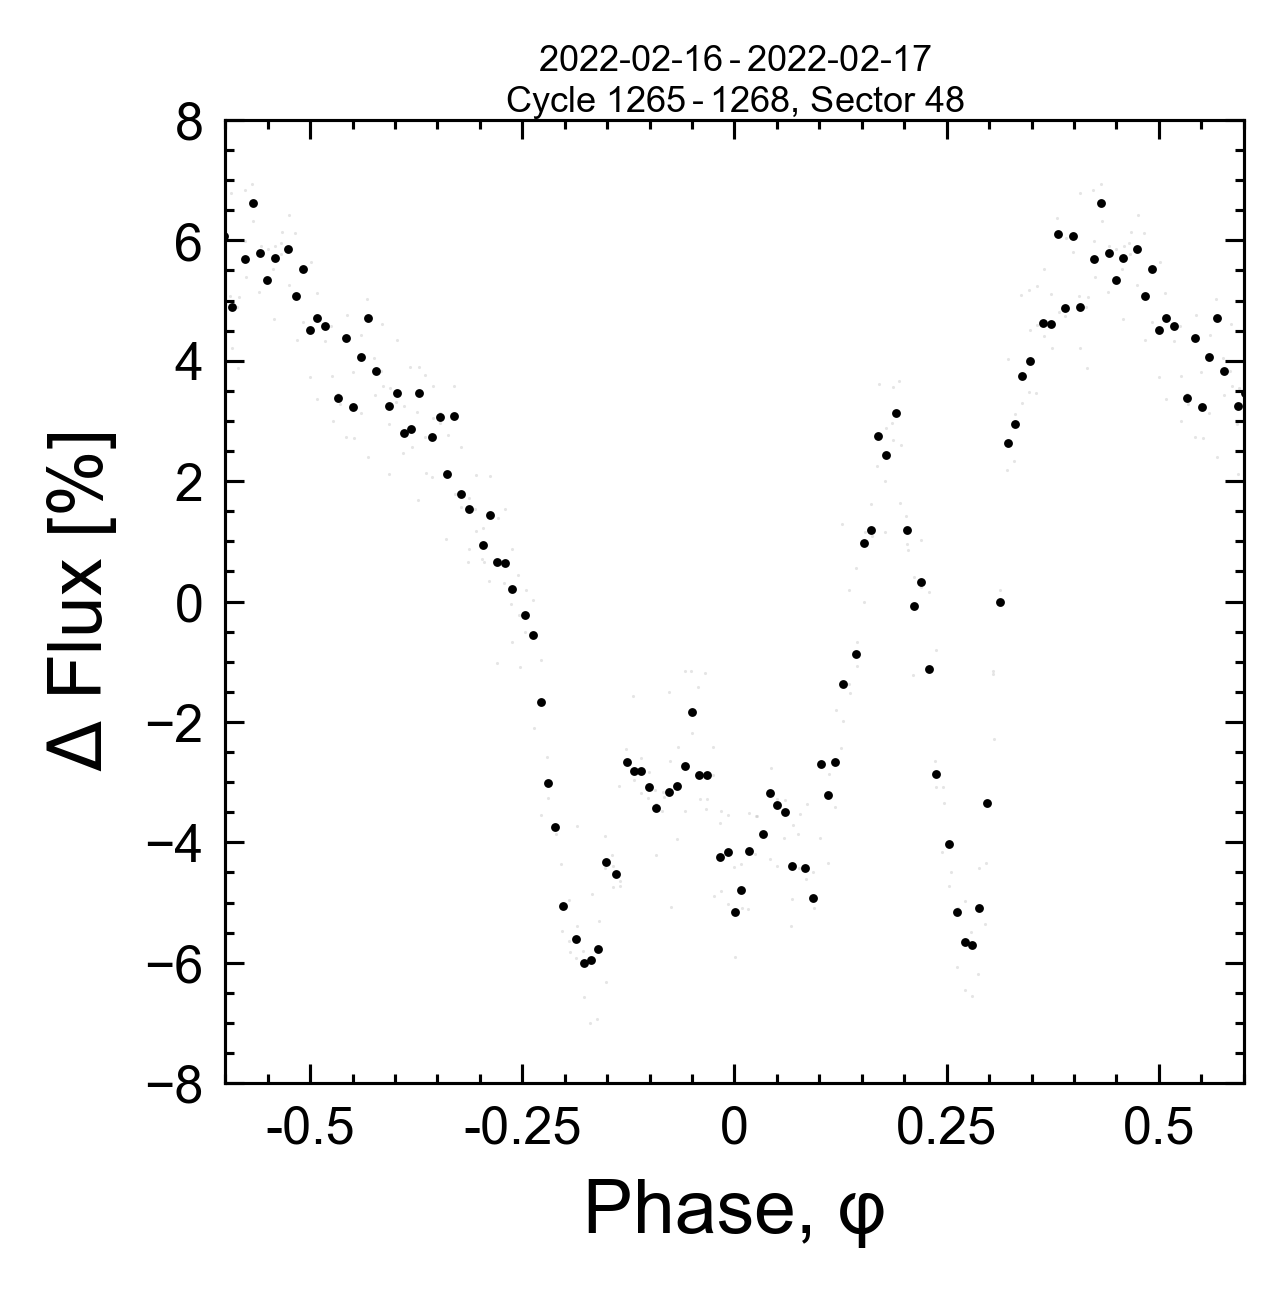
\includegraphics[width=0.7\textwidth]{figures/f1.png}
  \caption[]{{\bf Figure 1 (Movie):  TIC~141146667 is a complex periodic
  variable (CPV).} For the best experience, please view the online movie
  available
  \href{https://lgbouma.com/movies/movie_TIC1411_flux_phase.mp4}{here},
  which spans a baseline of 5{,}784 cycles irregularly sampled over three
  years.  The TESS light curve is phased to the \periodhr\ hour period in
  groups of a few cycles per frame.  This is the period both of
  stellar rotation, and (we hypothesize) of corotating clumps of
  circumstellar material.  Raw data acquired with two minute
  sampling are in gray; black is their average.  Similar to other members
  of this class, the sharp photometric features persist for tens to
  thousands of rotational cycles. }
  \label{fig:lc}
\end{figure}



The dearth of evidence for circumstellar material around CPVs is
surprising given that separate studies of young BAFGKM stars have, for
decades, reported that stellar coronae contain both hot ($10^6$ K) and
cool ($10^4$ K) plasma. In particular, time-series spectroscopy has
shown periodic high-velocity absorption and emission in Balmer lines
such as H$\alpha$, caused by long-lived, corotating clumps of cool
plasma (CITE, CITE, CITE).  Such clumps are forced into corotation by
the magnetic field, and the exact geometry of where the plasma can
accumulate is dictated by the magnetic field's topology.
For instance, a tilted dipole field tends to yield an accumulation
surface of a warped torus \cite{Townsend2005}, whereas in the limit of
a single strong discrete field line, accumulation occurs along a fixed
point \cite{Waugh2022}.  However, none of these stars have shown any
photometric anomalies (CITE), leaving open the issue of whether these
two separate areas of study have any direct connection.  Nonetheless,
CPVs do respond to sudden magnetic field changes: there are many
documented cases of otherwise long-lived eclipse features disappearing
immediately following stellar flares (CITE, CITE).

In this study, we present the first observations of corotating clumps
of cool plasma around a CPV.  We identified TIC~141146667 in previous
work \cite{Bouma2024} by searching the TESS two-minute data for stars
showing periodic variability with at least three sharp dips per cycle.  We
selected it from the resulting fifty high-quality CPVs for
spectroscopic observations because it was the brightest source for
which a full cycle could be observed in a half-night.  We observed it
for five hours on UT 2024-02-17 using the High Resolution Echelle
Spectrometer (HIRES; \cite{vogt_hires_1994}) on the Keck I 10m
telescope, roughly contemporaneous with TESS, which observed the star
from UT 2024-02-05 to UT 2024-02-26 with a duty cycle of XX\%.  In
detail, TESS was finishing a data downlink during the HIRES
observations, and photometric data collection resumed three rotation cycles
(12 hours) after the spectra were acquired.  Extended Data
Figure~\ref{fig:fulllc} shows the detailed photometric behavior of the
star before and after the exact epoch of observation; the star
remained sufficiently stable to not affect any of the interpretation
that follows.


\subsection{Results}

\begin{figure}[!tp]
  \centering
  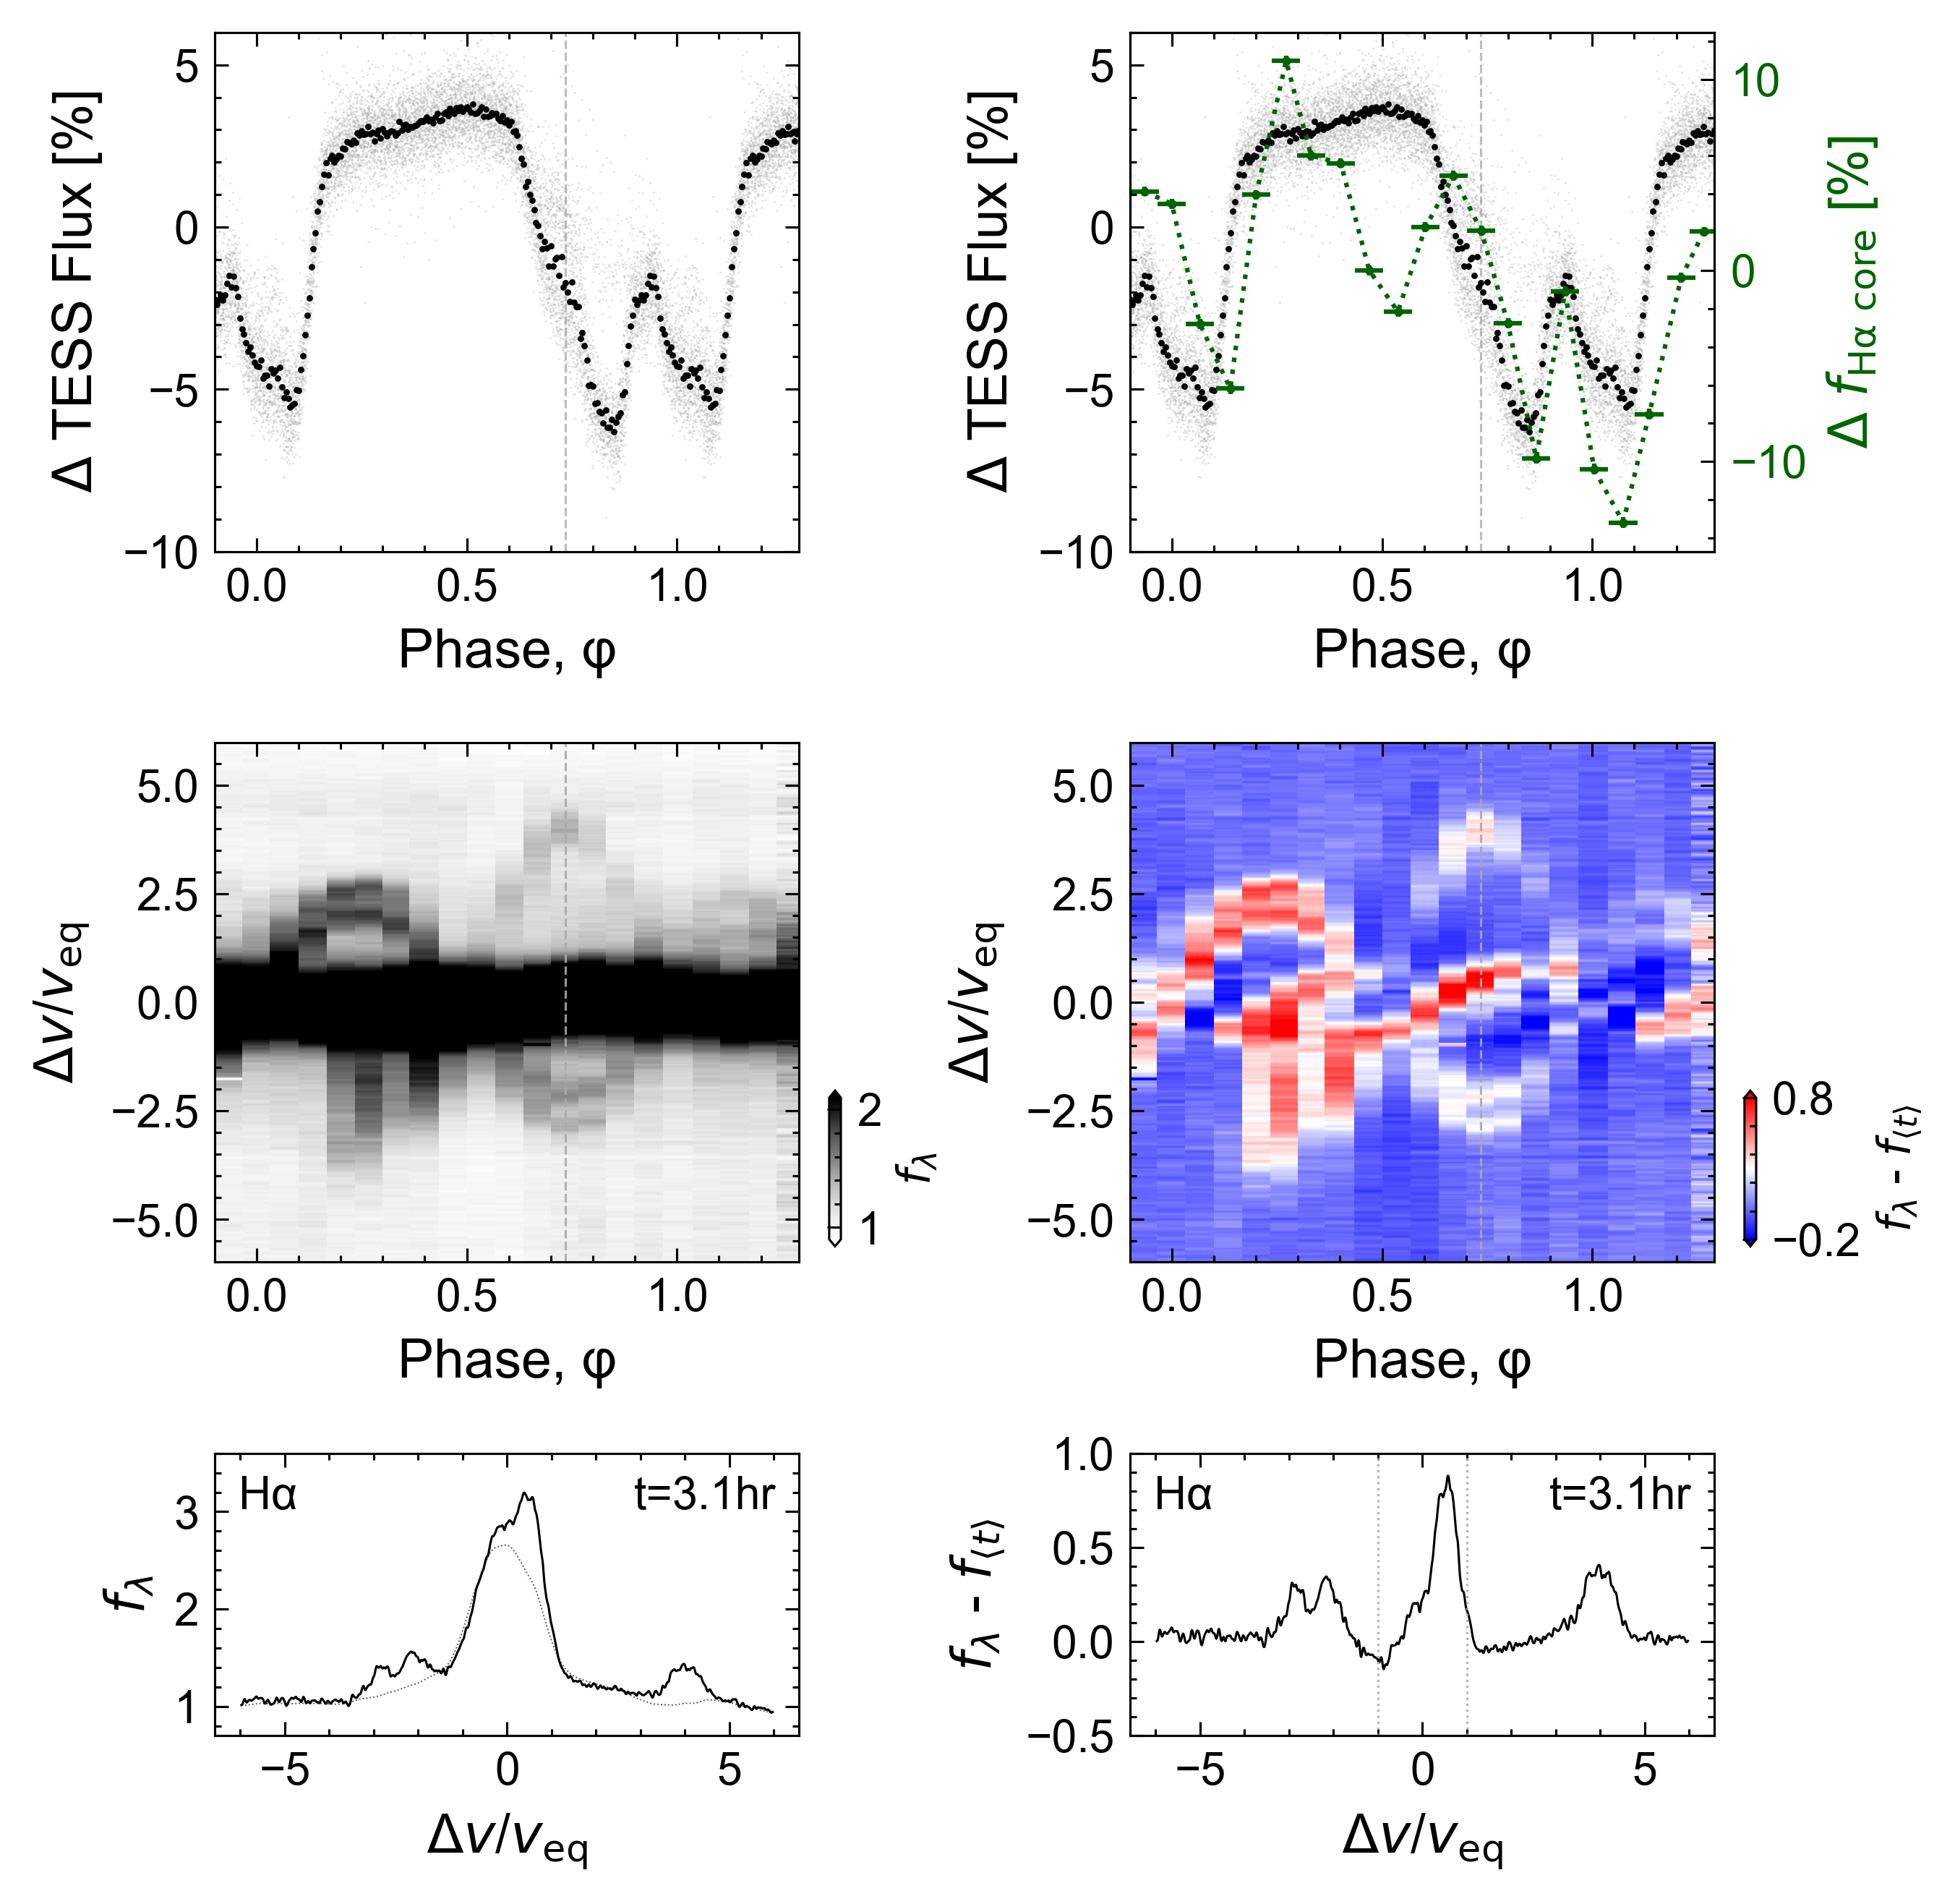
\includegraphics[width=0.99\textwidth]{figures/f2.png}
  \caption[]{{\bf Figure 2 (Movie):}  
  Hydrogen emission from circumstellar plasma orbiting TIC 141146667.
  {(\bf TODO)}For the best experience, please view the online movie
  available
  \href{https://lgbouma.com/movies/TIC141146667_sixpanel.mp4}{here}.
  {\bf Panel a:} TESS light curve from UT 2024-02-05 to UT
  2024-02-26 folded on the \periodhr\ hour period.  Black points are
  averaged; gray are the raw data.
  {\bf Panel b:} Keck/HIRES H$\alpha$ spectra
  acquired on UT 2024-02-17.  The continuum is set to unity, and the
  darkest color is set at twice the continuum to accentuate emission
  outside the line core ($|v/v_{\rm eq}|>1$, for $v_{\rm eq}$=130\,\kms).
  While emission in the line core originates in the stellar
  chromosphere, the sinusoidal emission features are most readily
  described by a warped plasma torus.
  {\bf Panel c:} Individual epochs of Panel b, visible in the
  online movie.  The dotted line shows a time-averaged spectrum,
  $f_{\langle t \rangle}$.
  {\bf Panel d:} As in Panel a, but overplotting the
  median-normalized H$\alpha$ light curve at $|v/v_{\rm eq}|<1$.
  {\bf Panel e:} As in Panel b, after subtracting the time-averaged
  spectrum. In addition to circumstellar emission, the line core shows
  absorption during the plasma clump transits.  The asymmetric stretch
  is set to match the dynamic range of the data.
  {\bf Panel f:} Individual epochs of Panel e, visible in the online
  movie.}
  \label{fig:spec}
\end{figure}

% photometry
Figure~\ref{fig:spec} shows the data from February 2024.  As expected
based on other CPVs \cite{Bouma2024}, the photometric shape of
TIC~141146667 evolved over the years following the 2022 discovery
data, while nonetheless remaining complex.  In February 2024, the
average photometric signal showed a gradual brightening over 45\% of
the period, followed by a complex eclipse-like feature spanning 55\%
of the period.  This eclipse-like feature shows two to three
local photometric minima, and one to two local maxima.

% ** keck/hires: emission beyond v/veq>1 (2-3 paragraphs)
The spectroscopy shows emission well outside the star's
equatorial velocity ($v_{\rm eq}$=130\,\kms).  There are at least two
distinct emission components, each spaced half a cycle apart in phase.  The
first has clearer sinusoidal behaviour and is double-peaked, with
semi-amplitudes of $K_1$=2.1\,$v_{\rm eq}$ and 2.7\,$v_{\rm eq}$.  The
flux excesses from these two peaks are correlated with one another,
with amplitudes varying from 100\% of the continuum flux early in the
observation sequence to 30\% by its end.  The component 180$^\circ$
opposite in phase is only detected from $\phi$=0.2-1.0, and 
from $\phi$=0.2-0.5, this latter component appears connected to the
star in velocity space.  While its peak semi-amplitude of
$K_1$=3.9\,$v_{\rm eq}$ is achieved at both $\phi$=0.25 and 0.75, its
amplitude decreases from a 60\% excess beyond the continuum to a 10\%
excess.   The sinusoidal period in all cases where emission is seen is
consistent with the photometric \periodhr\ hour period.  As we shall
discuss below, the only plausible explanation for the behavior at
$|\Delta v / v_{\rm eq}|>1$ is that circumstellar clumps of hydrogen
are corotating with the star.  These clumps transit in front of the
star when passing from negative to positive velocity.

% * keck/hires: absorption within v/veq<1
% * keck/hires: emission within v/veq<1
Within the stellar H$\alpha$ line core, at $|\Delta v / v_{\rm
eq}|<1$, the behavior is more complex.  Generally, one would
expect this region to be generated by the net superposition of bright
and dark regions on the stellar surface, and then modulated by any
occulting material capable of absorbing or emitting in H$\alpha$.  In
Figure~\ref{fig:spec}e, the behavior from $\phi$=0.4-1.2, is most easily
interpreted: from $\phi$=0.4-0.9, a hot region first gradually crosses
the stellar line profile, following from $\phi$=0.7-1.2 by the transit
of a cool region.  The phases $\phi$$<$0.4 seem to be a mix of similar
events, though the time sampling is sufficiently coarse that the
interpretation is less clear.
A final exercise to quantify the behavior in the line core is
shown in Figure~\ref{fig:spec}d, where $f_{\rm H\alpha\ core}$ denotes
the summed flux in the at $|\Delta v / v_{\rm eq}|<1$.
Changes in the line core flux are usually correlated with the
broadband variability, except at $\phi$=0.5, during the transit of the
higher-velocity clump and the occultation of the lower-velocity clump.


\subsection{Discussion}

The sinusoidal emission features require clumps of partially-ionized
hydrogen to be corotating with the star.
The velocity semi-amplitude of the sinusoids directly gives the
distance of these clumps from the stellar surface: 2.1-2.7\,$R_\star$
for one clump, and 3.9\,$R_\star$ for the other.
Their motion, rather than being Keplerian, can only be explained by
plasma being dragged along with the rotating stellar magnetic field.

The new data rule out two plausible origin scenarios for CPVs.
The ``starspot-only'' scenario \cite{Koen2021} has no means of
explaining this type of spectroscopic emission.
Similarly, a ``dust-only'' scenario in which the circumstellar
material would have a pure dust composition is also ruled out:
to explain the H$\alpha$ emission, the circumstellar clumps need to be
made of either a pure plasma, or a dusty plasma.
A priori, there are three plausible sources of such material:
the star, an old and undetected disk, or outgassing rocky bodies.

% * mass estimate
The density and mass of the material...

% TODO TODO: the rest!
* role of B: comparison to, and need for, RMHD models
  * massive B star / jupiter cnxn

* more wavelengths:
    Radio detection.   Relevance for B measurement.
    UV?  xray?
    need for jwst

* microphysics: the (probable) need for dust
    W1,W2,W3 no dust evidence.
    W4 detection questionable based on WISE images.




%%%%%%%%%%%%%%%%%%%%%%%%%%%%%%%%%%%%%%%%%%%%%%%%%%%%%%%%%%%%%%%%%%%%%%%%%%%%%%%
%%%%%%%%%%%%%%%%%%%%%%%%%%%%%%%%%%%%%%%%%%%%%%%%%%%%%%%%%%%%%%%%%%%%%%%%%%%%%%%

\newpage
\begin{methods}

\renewcommand{\figurename}{Extended Data Figure}
\renewcommand{\tablename}{Extended Data Table}
\setcounter{table}{0}  
\setcounter{figure}{0}  


\subsection{Observations}

\begin{figure}[!b]
  \centering
  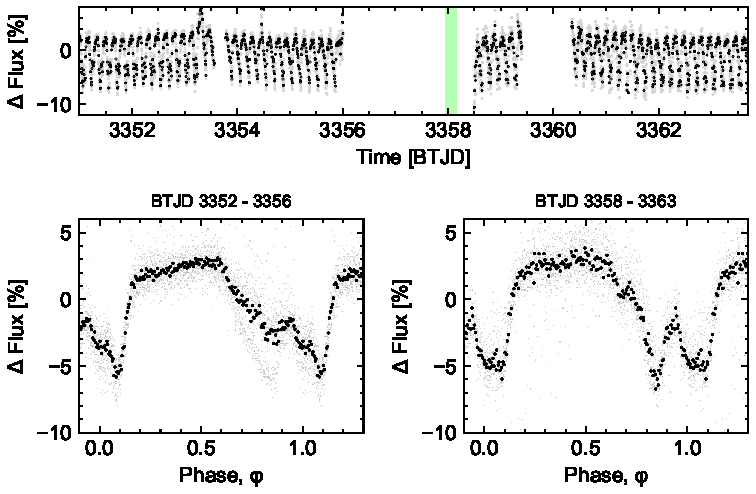
\includegraphics[width=0.99\textwidth]{figures/sf1.pdf}
  \caption{Detailed photometric evolution of TIC 141146667 near the
  epoch of spectroscopic observation (green). 
  {\bf Panel a}: Subset of TESS SAP\_FLUX acquired near time of
  Keck/HIRES observation.
  TESS downlinked data to the Deep Space Network from BTJD XXX to
  YYY, and was affected by scattered light from the Earth from BTJD
  3359.4 to 3360.15.
  %TODO: VERIFY!  Was it scattered light?  Or a legit flare?
  {\bf Panels b,c}: Folded light curve before and after spectroscopy.
  {\bf Panel d}: Zoom-in of Panel a, showing decreasing photometric
  scatter in the over three days (18 cycles).
  }
  \label{fig:fulllc}
\end{figure}

{\bf TESS:}

{\bf Keck/HIRES:}
We observed using the standard setup and reduction techniques of the
California Planet Survey \cite{Howard2010}.
Winds of 30 mph contributed to
1\farcs2$\pm$0\farcs2 seeing over the spectroscopic observations.  


\subsection{Data Reduction}

\subsection{Modeling the Emitting Clump}


%%%%%%%%%%%%%%%%%%%%%%%%%
% Supplementary Figures %
%%%%%%%%%%%%%%%%%%%%%%%%%

%%%%%%%%%%%%%%%%%%%%%%%%
% Supplementary Tables %
%%%%%%%%%%%%%%%%%%%%%%%%

% TEMPLATE: IRAS041
%
\begin{table}
    \centering
    \begin{tabular}{lcr}
    \hline 
    \hline
    Parameter & Host & Source \\
    \hline 
    \multicolumn{3}{c}{Identifiers} \\
    \hline
    TIC & 141146667 & TESS \\
    Gaia & todo & Gaia\ DR3 \\
    %2MASS & J04154278+2909597 & J04154269+2909558 & 2MASS \\
    %ALLWISE & J041542.77+290959.5 & ... & ALLWISE\\
    \hline
    \multicolumn{3}{c}{Astrometry} \\ 
    \hline
    $\alpha$ & todo & Gaia\ DR3 \\
    $\delta$ & todo & Gaia\ DR3 \\
    $\mu_{\alpha}$ (mas yr$^{-1}$ ) & todo & Gaia\ DR3 \\
    $\mu_{\delta}$ (mas yr$^{-1}$ ) & todo & Gaia\ DR3 \\
    $\pi$ (mas) & todo & Gaia\ DR3 \\
    \hline
    \multicolumn{3}{c}{Photometry} \\
    \hline
    $TESS$ (mag) & todo & TESS\ \\
    $G$ (mag) & todo & Gaia\ DR3 \\
    $G_{\rm BP}$ (mag) & todo & Gaia\ DR3\\
    $G_{\rm RP}$ (mag) & todo & Gaia\ DR3\\
    $J$ (mag) & todo & 2MASS\\
    $H$ (mag) & todo & 2MASS\\
    $K_s$ (mag) & todo & 2MASS\\
    $W1$ (mag) & todo & ALLWISE \\
    $W2$ (mag) & todo & ALLWISE \\
    $W3$ (mag) & todo & ALLWISE \\
    $W4$ (mag) & todo & ALLWISE \\
    \hline
    \multicolumn{3}{c}{Kinematics and Position} \\
    \hline
    $RV_{Bary}$ (km s$^{-1}$ ) & $13.35 \pm 3.39$ & Gaia\ DR3 \\
    $U$ (km s$^{-1}$ ) & & \\
    $V$ (km s$^{-1}$ ) & & \\
    $W$ (km s$^{-1}$ ) & & \\
    $X$ (pc)  & & \\
    $Y$ (pc)  & & \\
    $Z$ (pc) & & \\
    \hline
    \multicolumn{3}{c}{Physical Properties} \\
    \hline
    $P_{rot}$ (hours) & $3.930 \pm 0.XXX$ & This work \\ 
    $v \sin i_\star$(km s$^{-1}$) & todo & This work\\
    $i_\star$($^\circ$) & todo & This work \\
    $F_{bol}$ (erg cm$^{-2}$ s$^{-1}$ ) & todo & This work\\
    $T_{eff}$ (K) & todo & This work\\
    $A_V$ (mag) & todo & This work \\
    $R_\star$ ($R_{\odot}$) & todo & This work\\
    $L_\star$ ($L_{\odot}$)  & todo & This work\\
    $M_\star$ ($M_{\odot}$)  & todo & This work\\
    Age (Myr) & todo &  This work \\
    \hline
    \end{tabular}
    \caption{Properties of \starname.}
    \label{tab:stellarParameters}
\end{table}


\end{methods}

\bibliography{cpvbib.bib} % common bib file
\bibliographystyle{naturemagfixed}   


\begin{addendum}

\item[Acknowledgments] The author thanks X, Y, Z.
  L.G.B. was suported by...
	Acknowledge TESS...


%TC:ignore
%% Author Contribution
\item[Author Contributions] ...
%TC:endignore

\item[Data Availability] ...

\item[Competing Interests] The authors declare that they have no competing
financial interests.
 
\item[Correspondence] Correspondence and requests for materials should be
addressed to ...
 
\item[Code availability] We provide access to a GitHub repository including all
code created for the analysis of this project that is not already publicly
available.

\end{addendum}



\end{document}


